% !TeX root = 机械设计.tex
% ============================================================
%  第六章 带传动
%  来源：《5.带传动.md》笔记与课件《08带传动》整理
% ============================================================
\chapter{带传动}
\label{chap:带传动}

\section{概述}
\label{sec:带传动:概述}

\subsection{带传动的工作原理及特点}
\label{sec:带传动:工作原理及特点}

\textbf{组成}：主动带轮、从动带轮、传动带。

\textbf{工作原理}：依靠带与带轮接触面间的摩擦力拖动从动轮一起回转。

\begin{figure}[htbp]
	\centering
	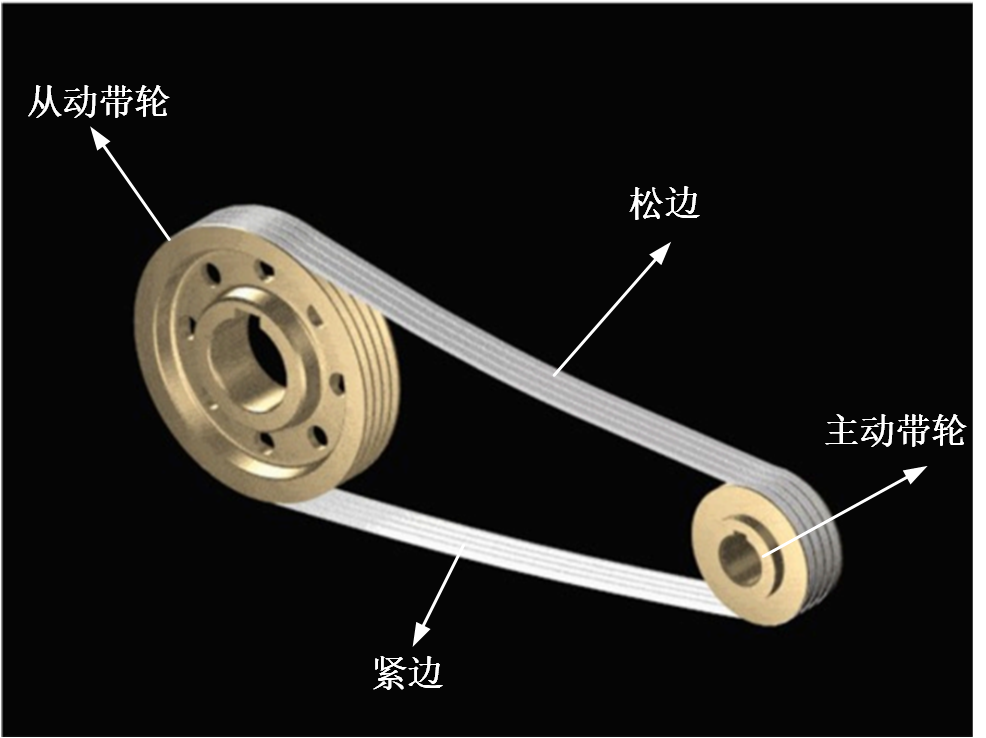
\includegraphics[width=0.7\textwidth]{Figure/传送带组成.png}
	\caption{带传动的组成}
	\label{fig:带传动:组成}
\end{figure}

\textbf{优点}：
\begin{enumerate}
	\item 有良好的\textbf{挠性}和\textbf{弹性}，有吸振和缓冲作用，可使带传动平稳、噪声小；
	\item 有\textbf{过载保护作用}：过载时带在带轮上发生相对滑动，可防止其他零件的损坏；
	\item 结构简单，制造、安装、维护方便；
	\item 适用于两轴\textbf{中心距较大}的传动（最大距离可达 $15$ m）。
\end{enumerate}

\textbf{缺点}：
\begin{enumerate}
	\item 由于弹性滑动，使传动效率降低，不能保证准确的传动比；
	\item 由于带传动需要初始张紧，当传递同样大的圆周力时，与啮合传动相比轴上的压力较大；
	\item 结构尺寸较大，不紧凑；
	\item 传动带寿命较短；
	\item 传动带与带轮之间会产生摩擦放电现象，不宜用于有爆炸危险的场合。
\end{enumerate}

\begin{note}
	上述优缺点均可由后面的受力分析、应力分析与弹性滑动分析一一回溯。
\end{note}

\subsection{带传动的类型与应用}
\label{sec:带传动:类型与应用}

\begin{table}[H]
\centering
\small
\setlength{\tabcolsep}{4pt}
\caption{带传动的类型与应用}
\label{tab:带传动:类型与应用}
\begin{tabular}{p{2.6cm}p{5.0cm}p{6.0cm}}
	\toprule
	类型 & 结构 / 工作原理 & 特点与应用 \\
	\midrule
	平带传动 & 带为扁平矩形截面，靠带与带轮面间的摩擦工作 & 最简单，适合于中心距较大的情况 \\
	V 带传动（三角带） & 靠两侧边与轮槽接触，靠两侧面产生的摩擦力工作 & 摩擦力比平带大，能传递较大的功率 \\
	多楔带传动 & 由若干条 V 形楔组成 & 适用于传递功率较大、要求结构紧凑的场合 \\
	同步带传动 & 啮合型：靠带上的齿与轮缘上的齿相互啮合传动 & 传动比恒定，柔韧性好，张紧力小，带比较轻薄，在高速设备、数控机床、机器人行业、汽车行业、轻纺行业中广泛应用 \\
	\bottomrule
\end{tabular}
\end{table}

V 带靠两侧边与轮槽接触，靠两侧面所产生的摩擦力来工作。当带被张紧时，带以力 $Q$ 压向轮槽，两侧面的法向力为
\begin{equation}
	2N\sin\frac{\varphi}{2}=Q
	\quad\Longrightarrow\quad
	N=\frac{Q}{2\sin(\varphi/2)},
	\label{eq:带传动:V带法向力}
\end{equation}
摩擦力为
\begin{equation}
	F_f=2fN=\frac{fQ}{\sin(\varphi/2)}=f_vQ,\qquad
	f_v=\frac{f}{\sin(\varphi/2)},
	\label{eq:带传动:V带摩擦力}
\end{equation}
其中：
\begin{itemize}
	\item $f_v$ 为当量摩擦因数；
	\item $\varphi$ 为 V 带带轮轮槽楔角。
\end{itemize}
所以 V 带传动的摩擦力比平带大，能传递较大的功率。

\begin{figure}[htbp]
	\centering
	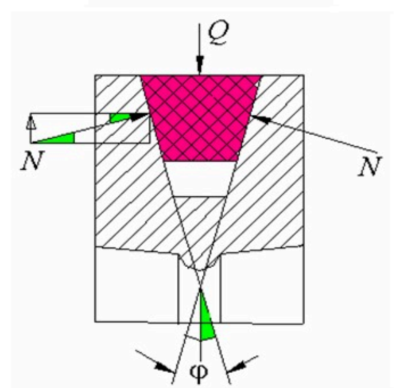
\includegraphics[width=0.6\textwidth]{Figure/V带的摩擦受力分析.png}
	\caption{V 带的摩擦受力分析}
	\label{fig:带传动:V带受力}
\end{figure}

\subsection{V 带及其标准}
\label{sec:带传动:V带及其标准}

V 带的主要参数：
\begin{itemize}
	\item 中性层（节面）；
	\item 带轮基准直径 $D$；
	\item 基准长度 $L_d$（公称长度）；
	\item 标注示例：A2240——A 型带，公称长度 $L_d=2240$ mm。
\end{itemize}

普通 V 带是标准件，截面形状为楔角 $40^{\circ}$ 的梯形。按截面尺寸由小到大分为 Y、Z、A、B、C、D、E 七种：截面尺寸越大，承载能力越大，适用的传动转速越低。

V 带轮的最小基准直径见表~\ref{tab:带传动:最小基准直径}（教材表 8-4）。

\begin{table}[H]
\centering
\small
\setlength{\tabcolsep}{4pt}
\caption{V 带轮的最小基准直径}
\label{tab:带传动:最小基准直径}
\begin{tabular}{l *{10}{c}}
	\toprule
	带型 & Z & SPZ & A & SPA & B & SPB & C & SPC & D & E \\
	\midrule
	$d_{d\min}$/mm & 50 & 63 & 75 & 90 & 125 & 140 & 200 & 224 & 355 & 500 \\
	\bottomrule
\end{tabular}
\end{table}

\section{带传动的工作情况分析}
\label{sec:带传动:工作情况分析}

带传动的一些基本参数如图~\ref{fig:带传动:参数示例} 所示。

\begin{figure}[htbp]
	\centering
	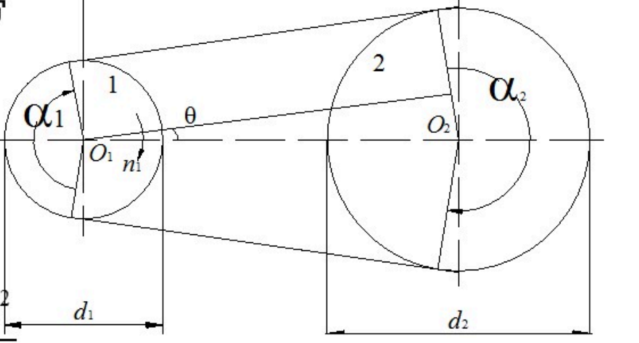
\includegraphics[width=0.75\textwidth]{Figure/带传动各参数示例.png}
	\caption{带传动各参数示例}
	\label{fig:带传动:参数示例}
\end{figure}

\subsection{带传动的受力分析}
\label{sec:带传动:受力分析}

工作前，两边初拉力均为 $F_0$；工作时，两边拉力变化：紧边 $F_0\rightarrow F_1$，松边 $F_0\rightarrow F_2$。

由工作时带的总长度不变（紧边伸长的量等于松边缩短的量），有
\begin{equation}
	F_1-F_0=F_0-F_2
	\quad\text{或}\quad
	F_1+F_2=2F_0.
	\label{eq:带传动:紧松边拉力}
\end{equation}
取主动轮上的一段带为分离体，总摩擦力 $F_e$ 和两边拉力对轴心的力矩代数和 $\sum T=0$，得
\begin{equation}
	F_e=F_1-F_2,
	\label{eq:带传动:有效拉力}
\end{equation}
$F_e$ 称为带的有效拉力，即带与带轮接触面上各点摩擦力的总和。

带传动所能传递的功率为
\begin{equation}
	P_{\mathrm{kW}}=\frac{F_e v}{1000},
	\label{eq:带传动:功率}
\end{equation}
式中 $F_e$ 的单位为 N，$v$ 的单位为 m/s，$P_{\mathrm{kW}}$ 的单位为 kW。

\subsection{带传动的最大有效拉力及其影响因素}
\label{sec:带传动:最大有效拉力}

承受载荷越大，摩擦力越大；当带沿带轮有打滑趋势时，摩擦力达到最大值，带的有效拉力也达到最大值。此时 $F_1$ 与 $F_2$ 的关系为
\begin{equation}
	\frac{F_1}{F_2}=\mathrm{e}^{f\alpha},
	\label{eq:带传动:欧拉公式}
\end{equation}
其中 $f$ 为摩擦因数，$\alpha$ 为包角（单位 rad）。

包角（小带轮包角 $\alpha_1$）为
\begin{equation}
	\alpha_1=180^{\circ}-\frac{D_2-D_1}{a}\times 60^{\circ},\qquad
	\alpha_2=180^{\circ}+\frac{D_2-D_1}{a}\times 60^{\circ}.
	\label{eq:带传动:包角}
\end{equation}

将 $F_1+F_2=2F_0$ 代入上式，可得带所能传递的最大有效拉力（即有效拉力的临界值）
\begin{equation}
	F_{ec}=2F_0\frac{\mathrm{e}^{f\alpha}-1}{\mathrm{e}^{f\alpha}+1}
	=2F_0\frac{1-1/\mathrm{e}^{f\alpha}}{1+1/\mathrm{e}^{f\alpha}}.
	\label{eq:带传动:最大有效拉力}
\end{equation}

\begin{warnbox}[打滑条件]
	由功率算得的有效拉力超过临界值时发生打滑，即
	\[
	F_e>F_{ec}.
	\]
\end{warnbox}

\subsection{带的应力分析}
\label{sec:带传动:应力分析}

带在工作时产生三种应力：
\begin{enumerate}
	\item \textbf{拉应力}：紧边 $\sigma_1=F_1/A$；松边 $\sigma_2=F_2/A$。
	\item \textbf{弯曲应力}：带绕在带轮上时要引起弯曲应力
	      \begin{equation}
		      \sigma_b\approx\frac{Eh}{D},
		      \label{eq:带传动:弯曲应力}
	      \end{equation}
	      其中 $h$ 为带的横截面厚度，$D$ 为带轮的计算直径，$E$ 为带的弹性模量。
	\item \textbf{离心应力}：
	      \begin{equation}
		      \sigma_c=\frac{qv^2}{A},
		      \label{eq:带传动:离心应力}
	      \end{equation}
	      其中 $q$ 为带单位长度的质量，$v$ 为带的线速度。
\end{enumerate}

三种应力中：紧边拉应力大于松边拉应力；带轮直径越小弯曲应力越大；离心应力近似全局相同。于是瞬时最大应力在\textbf{紧边开始绕上小带轮处}，此时的最大应力可近似表示为
\begin{equation}
	\sigma_{\max}=\sigma_1+\sigma_{b1}+\sigma_c.
	\label{eq:带传动:最大应力}
\end{equation}

带是在变应力下工作，所以带的疲劳寿命取决于 $\sigma_{\max}$ 与应力循环次数 $N$；当 $N$ 达到一定数值后，带产生疲劳损坏。疲劳强度条件为
\begin{equation}
	\sigma_{\max}=\sigma_1+\sigma_{b1}+\sigma_c\le[\sigma]
	\quad\Rightarrow\quad
	\sigma_1\le[\sigma]-\sigma_{b1}-\sigma_c.
	\label{eq:带传动:疲劳强度条件}
\end{equation}

讨论：
\begin{enumerate}
	\item $\sigma_c=qv^2/A$，$q$ 为单位长度质量，$v$ 增大则 $\sigma_c$ 增大。对于高速带，$\sigma_c$ 对带的寿命起主要作用。
	\item V 带传动中，$\sigma_{b1}$ 对寿命起主要作用，所以要限制小带轮的最小基准直径 $D_{\min}$（教材表 8-4）。
\end{enumerate}

\subsection{带的弹性滑动和打滑}
\label{sec:带传动:弹性滑动和打滑}

\begin{definition}[弹性滑动]
	由于带的弹性变形引起的带与带轮之间的（微量）相对滑动，称为\textbf{弹性滑动}。
\end{definition}

弹性滑动是带传动工作的固有特性，是\textbf{不可避免}的。弹性滑动与紧、松边拉力值有关：带传递的圆周力 $F_e$ 越大，弹性滑动越大。

\begin{definition}[打滑]
	由过载引起的带与带轮发生的相对滑动称为\textbf{打滑}。
\end{definition}

打滑使带磨损加剧，从动轮转速急剧下降，甚至传动失效。

\begin{table}[H]
\centering
\small
\setlength{\tabcolsep}{4pt}
\caption{弹性滑动与打滑的对比}
\label{tab:带传动:弹性滑动与打滑}
\begin{tabular}{p{2.2cm}p{5.6cm}p{5.6cm}}
	\toprule
	对比项 & 弹性滑动 & 打滑 \\
	\midrule
	产生原因 & 带的弹性变形引起 & 过载引起（外载荷超过最大有效圆周力） \\
	性质 & 固有特性，不可避免 & 可以避免的失效形式 \\
	滑动范围 & 局部、微量 & 沿带轮面全面滑动 \\
	后果 & 传动比不准确、传动效率降低 & 带磨损加剧，从动轮转速急剧下降，甚至传动失效 \\
	\bottomrule
\end{tabular}
\end{table}

\textbf{滑动率与传动比}。滑动率为
\begin{equation}
	\varepsilon=\frac{v_1-v_2}{v_1}\times 100\%,
	\label{eq:带传动:滑动率}
\end{equation}
或 $v_2=(1-\varepsilon)v_1$，其中带速
\begin{equation}
	v=\frac{\pi Dn}{60\times 1000}.
	\label{eq:带传动:带速}
\end{equation}
代入滑动率公式，可得 $D_2n_2=(1-\varepsilon)D_1n_1$，因而带传动的实际平均传动比为
\begin{equation}
	i=\frac{n_1}{n_2}=\frac{D_2}{D_1(1-\varepsilon)}.
	\label{eq:带传动:传动比}
\end{equation}
在一般传动中，因滑动率不大（$\varepsilon=1\%\sim2\%$），故可不予考虑，而取传动比为
\begin{equation}
	i=\frac{n_1}{n_2}\approx\frac{D_2}{D_1}.
	\label{eq:带传动:近似传动比}
\end{equation}

\section{V 带传动的设计计算}
\label{sec:带传动:设计计算}

\subsection{设计准则和单根 V 带的基本额定功率}
\label{sec:带传动:设计准则}

失效形式：1）打滑；2）带的疲劳破坏；另外还有磨损、静载拉断等。

设计准则：保证带在不打滑的前提下，具有足够的疲劳强度和寿命。

单根 V 带的基本额定功率 $P_0$ 是根据特定的实验和分析确定的，是 V 带传动设计的主要依据：
\begin{itemize}
	\item 由临界条件（带处于打滑趋势）确定带的最大有效拉力 $F_e$，单根 V 带所传递的临界功率 $P_0=F_e v/1000$；
	\item 由疲劳强度条件 $\sigma_1\le[\sigma]-\sigma_{b1}-\sigma_c$ 限定单根带所能传递的功率。
\end{itemize}

实验条件：包角 $\alpha=180^{\circ}$、特定长度、平稳的工作载荷。单根 V 带的基本额定功率 $P_0$ 见教材表 8-6(a)。

\subsection{V 带传动的设计步骤和方法}
\label{sec:带传动:设计步骤}

已知条件：$P$、$n_1$、$n_2$ 或 $i$，传动布置要求（中心距 $a$），工作条件。

设计要求：带——型号、根数、长度；轮——$D_{\min}$、结构、尺寸；中心距 $a$、轴压力 $Q$ 等。

设计步骤：

\begin{enumerate}
	\item \textbf{确定计算功率 $P_{ca}$}：
	      \begin{equation}
		      P_{ca}=K_AP,
		      \label{eq:带传动:计算功率}
	      \end{equation}
	      其中 $P$ 为额定功率（kW），$K_A$ 为工况系数（教材表 8-7）。

	\item \textbf{选择带型号}：根据计算功率 $P_{ca}$、小带轮转速 $n_1$ 按选型图选取普通 V 带型号（教材图 8-7）。

	\item \textbf{确定带轮直径（验算带速 $v$）}：
	      \begin{itemize}
		      \item 根据带的型号选择小带轮基准直径 $D_1$，一般应 $D_1\ge D_{d\min}$（教材表 8-4）；
		      \item 大带轮直径：考虑滑动率时 $D_2=\dfrac{D_1n_1(1-\varepsilon)}{n_2}$，不考虑滑动率时 $D_2=\dfrac{D_1n_1}{n_2}$；
		      \item 验算带速：
		            \begin{equation}
			            v=\frac{\pi D_1n_1}{60\times 1000},
			            \label{eq:带传动:验算带速}
		            \end{equation}
		            要求最佳带速 $v=20\sim25$ m/s；
		      \item 讨论：
		            \begin{itemize}
			            \item $v$ 太小：由 $P=Fv$ 可知，传递同样功率时圆周力 $F$ 太大，带寿命下降；
			            \item $v$ 太大：离心力大，带与带轮正压力减小，摩擦力减小，传递载荷能力下降；
			            \item 如 $v$ 不合适，应重选 $D_1$。
		            \end{itemize}
	      \end{itemize}

	\item \textbf{求中心距 $a$ 和带的基准长度 $L_d$}：
	      \begin{itemize}
		      \item 初选 $a_0$：$0.7(D_1+D_2)<a_0<2(D_1+D_2)$；
		      \item 由 $a_0$ 定计算基准带长度：
		            \begin{equation}
			            L_{d0}\approx 2a_0+\frac{\pi}{2}(D_1+D_2)+\frac{(D_2-D_1)^2}{4a_0};
			            \label{eq:带传动:基准长度初值}
		            \end{equation}
		      \item 根据 $L_{d0}$ 按教材表 8-3 选定相近的基准长度 $L_d$；
		      \item 由 $L_d$ 求实际中心距：
		            \begin{equation}
			            a\approx a_0+\frac{L_d-L_{d0}}{2};
			            \label{eq:带传动:实际中心距}
		            \end{equation}
		      \item 考虑安装、中心距调整、补偿张紧力 $F_0$，中心距 $a$ 的变动范围为
		            \begin{equation}
			            (a-0.015L_d)\sim(a+0.03L_d).
			            \label{eq:带传动:中心距变动范围}
		            \end{equation}
	      \end{itemize}

	\item \textbf{验算小轮包角}：
	      \begin{equation}
		      \alpha_1=180^{\circ}-\frac{D_2-D_1}{a}\times 60^{\circ}\ge 120^{\circ}
		      \quad(\text{个别情况下至少}\ 90^{\circ}).
		      \label{eq:带传动:验算包角}
	      \end{equation}
	      如不满足，采取的措施为：增大中心距；加张紧轮。

	\item \textbf{计算带的根数 $z$}：
	      \begin{equation}
		      z=\frac{P_{ca}}{(P_0+\Delta P_0)K_\alpha K_L K},
		      \label{eq:带传动:根数}
	      \end{equation}
	      其中：
	      \begin{itemize}
		      \item $K_\alpha$：包角系数，查教材表 8-9；
		      \item $K_L$：长度系数，查教材表 8-10；
		      \item $\Delta P_0$：考虑 $i\neq1$ 时传动功率的增量，见教材表 8-6(b)；
		      \item $K$：材质系数；
		      \item $P_0$：单根 V 带的基本额定功率，见表 8-6(a)。
	      \end{itemize}

	\item \textbf{确定带的初拉力 $F_0$（单根带）}：
	      \begin{equation}
		      F_0=500\frac{P_{ca}}{zv}\left(\frac{2.5}{K_\alpha}-1\right)+qv^2.
		      \label{eq:带传动:初拉力}
	      \end{equation}

	\item \textbf{求带作用于轴的压力 $Q$}：
	      \begin{equation}
		      Q=2zF_0\sin\frac{\alpha_1}{2}.
		      \label{eq:带传动:轴压力}
	      \end{equation}
\end{enumerate}

\section{V 带轮的设计}
\label{sec:带传动:带轮设计}

\subsection{设计要求}
\label{sec:带传动:带轮设计要求}

重量轻，结构工艺性好，无过大的铸造内应力，质量分布均匀；轮槽表面要经过精细加工，以减轻带的磨损；各轮槽尺寸与角度要有一定的精度，使载荷分布较均匀。

\subsection{带轮材料}
\label{sec:带传动:带轮材料}

铸铁（常用）、铸钢（转速 $v$ 较大时）、铸铝或塑料（重量轻，小功率传动）。

\subsection{带轮的结构尺寸}
\label{sec:带传动:带轮结构尺寸}

按直径大小可做成实心式、腹板式和轮辐式；实心式用于 $D\le(2.5\sim3)d$（$d$ 为轴的直径）。

\section{带传动的张紧与维护}
\label{sec:带传动:张紧与维护}

\subsection{带的张紧}
\label{sec:带传动:张紧}

初拉力 $F_0$ 太小，传动能力下降；$F_0$ 太大，带寿命下降，应保证要求的初拉力。

常用的张紧方法：
\begin{enumerate}
	\item 调节中心距；
	\item 张紧轮。
\end{enumerate}

张紧轮位置：① 松边内侧、靠大带轮；② 松边外侧（用于增大小带轮包角）。

\subsection{带的维护}
\label{sec:带传动:维护}

\begin{enumerate}
	\item 安装时，最好先缩小中心距，后套上 V 带，再预调整使带张紧，不能硬撬，以免损坏胶带，降低使用寿命；
	\item 禁止与矿物油、酸、碱等介质接触，以免腐蚀带，亦不能曝晒；
	\item 带根数较多的传动，若少数几根破坏，不要立即补全，否则由于旧带已永久变形，新旧带一起使用，载荷分配不均，加速新带的损坏，应使旧带继续工作或全部换新；
	\item 为保证安全生产，应安装防护罩；
	\item 带工作一段时间后，应重新张紧。
\end{enumerate}

\section{同步带传动}
\label{sec:带传动:同步带}

同步带传动靠挠性带上的齿和轮缘上的齿相互啮合进行传动。

特点：保证准确的传动比；张紧力小；重量轻；柔韧性好；制造安装要求高。

\section*{本章重点}
\addcontentsline{toc}{section}{本章重点}

\begin{enumerate}
	\item 带传动的组成、工作原理与优缺点；
	\item 受力分析：$F_e=F_1-F_2$、$F_1+F_2=2F_0$；
	\item 最大有效拉力 $F_{ec}$ 与打滑条件；
	\item 带的三种应力、瞬时最大应力位置与疲劳强度条件；
	\item 弹性滑动与打滑的区别；
	\item 滑动率与传动比；
	\item V 带传动的设计步骤：计算功率、带型、带轮直径与带速、中心距与基准长度、包角、根数、初拉力、轴压力；
	\item 带传动的张紧方法与维护。
\end{enumerate}
